\documentclass[main.tex]{subfiles} 

\begin{document}
\section*{Analyse}
\label{sec:2}

Hvordan ble undervisningen lagt opp for å skape god begrepsforståelse i naturfagstimene?

Både til den første og andre timen ble dialog initiert av læreren. Helklassesamtalene hadde preg av
IRE/F metoden, m.a.o lærer tar initiativ(I), elev responderer(R) og responsen blir evaluert(E) 
og/eller kommentert(F - feedback). Til den første timen rekker elevene opp hånda for å 
respondere. Det viser seg at det er noen få elever som er villig til å svare. 


\citeA[s. 176]{klet13} referer til et studie når hun viser til viktigheten av at lærerne 
legger til rette for \emph{systematisk trening, øvelse og bruk av naturfaglige begreper for å utvikle 
elevenes naturfaglige forståelse, inkludert repitisjon av sentrale begreper.}

Ved å være bevisst på at alle elevene skal ha kjennskap til 
begrepene som blir tatt opp og repetert, er det da nødvendig å få bekreftet at elevene innehar en 
overordnet forståelse. Det kan derfor være nødvendig å utpeke noen elever som ikke viser aktiv 
deltagelse i timen og frembringe deres respons. Hvis elevene ikke klarer å respondere på lærer 
initiativ, kan utspørringen av elevene vise hull i deres kunnskap. I 2. timen ble denne formen for
utspørringen anvendt til å frembringe respons. Til denne timen brukte jeg navnekort, hvor en elevs navn 
ble opplest vilkårlig fra en usortert liste, og deretter fikk eleven ordet og tid til å respondere. 
Elevrespons ble enten akseptert, eller hvis eleven viste svakheter i sin forståelse ble spørsmålet 
gitt til andre i klassen. Dialogen ble avsluttet med en vurdering og/eller oppsummering, og hvis 
nødvendig ble tilleggsinformasjon supplert. 

Ved å forutse elevsvar før elever i klassen blir initiert, kan misforståelser som ofte oppstår bli redegjort
av læreren, og respons som ofte opptrer kan tas stilling til. Dette krever derimot en god del erfaring fra 
læreren sin side. I \citeA[s. ~401]{batp08} klassifiseres dette som \emph{knowledge of content and students, (KCS)}.
Over tid vil en lærer danne omfattende KCS og dette kan dermed bidra til å øke kvaliteten på helklassesamtalene.

\citeA[s. ~136]{klet13} beskriver en god undervisningsseksens der lærere klarer å balansere mellom tilegnelses-,
utprøvings-, og konsolideringssituasjoner. Ifølge Klette har norske klasserom ensidige tendenser i bruken av 
variert arbeidsmåter. Slik det kan ses fra figur \ref{fig:odeg10}, er det for eksempel lite konsolideringssituasjoner.
Lærernes metalæringsaktiviteter regnes som særlig avgjørende for å sikre elevenes læring (\citeNP[s. 186]{klet13}). Derimot å bruke dette som et fast
organiserende prinsipp, blir sjelden gjennomført (\citeNP[s. 26]{odeg10}).
Gjennom alle timene har aktivering av forkunnskaper, gjennom repitisjon og gjenbruk av begreper og gjennomgang av 
lekser, bruk av appetittvekker, som i vår tilfellet kan være bruken av en anatomisk modell og observasjon av
encellede organismer gjennom et mikroskop, og til slutt oppsummering av timen med gjentagelse av prosessen
for flercellede organismer i motsatt rekkefølge, fra organismer med organsystemmer til encellede organismer, har 
alle timene bæret preg av bevisst fokus på bruk av konsolideringssituasjoner/metalæringsaktiviteter. 


Fra figuren \ref{fig:odeg10} kan vi også se at i en vanlig naturfagstime brukes mye tid på å utvikle nytt fagstoff.
Det kan nok påstås at undervisningsopplegget hadde et preg av mange fagtermer, men fokuset i undervisningen var ikke
på å innføre fagtermene, men isteden var fokuset å danne forståelse om begrepene og deres sammenhenger. 

\begin{figure}[h!]
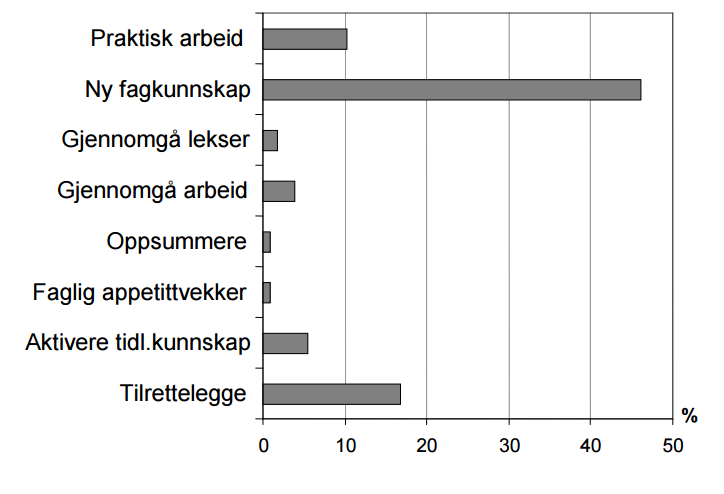
\includegraphics[scale = 0.6]{../figures/undervisnings_aktivitet.png}
\caption{Oversikt over naturfaglærernes undervisningstilbud til elevene fra PISA+ studie. Kilde: \protect\citeA{odeg10}.}
\label{fig:odeg10}
\end{figure}

%gode fagsentrerte samtaler mellom elever hvor elever brukte egne erfaringer
%og språket for å oppnå faglig forståelse, eller faglige samtaler med lærer som hjelper til å skape
%bro mellom praksis og teori 
%\citeA{odeg10}


%  ”inquiry-based science teaching” 
%\citeA{knai11}

Siden resterende del av timen skal brukes til repetisjon, er det ikke nødvendig å 
prøve å finne svakheter i elevenes respons gjennom helklassesamtalen. For å finne slike svakheter 
ble gruppesamtalene en bedre plattform. I den forbindelse ble tokolonnenotatet tatt i bruk (se 
vedlegg : \ref{sec:tokolonnenotat}).

Evnen til abstrahering henger ifølge Vygotsky (\citeNP[s. 127]{bta98}) med begrepsundervisning, som en
form for vitenskapeliggjøring av hverdagsbegreper. Hvis elever ikke har god begrepsforståelse
kan de ende opp med å bruke naturvitenskapelige begreper i feil kontekst og danne feil 
forbindelser med begrepene. Dette avhenger av deres forkunnskaper. Ausubels kognitive bruer 
(\citeNP[s. 71]{math15}), hans teori om begrepslæring på høyere nivå og hvordan læreren best kan legge 
til rette for slik læring og bruk av begrepene,  handler om å danne forbindelser mellom undervisningsmateriell
og relevante ideer i elevenes kognitive struktur.

Blant hovedområder i naturfag 1.-10. trinn inkluderer det \emph{Forskerspiren}, \emph{Mangfold i naturen} og \emph{Kropp og helse}. Undervisningsopplegget er laget etter kompetansemål fra de første to hovedområdene. Dessuten har undervisningsopplegget koblingen til den siste hovedområdet \emph{Kropp og helse}. Hos Utanningsdirektoratet står det blant annet at
\begin{displayquote}
Hovedområdet dreier seg om hvordan kroppen er bygd opp, påvirkes og endres over tid. Kunnskap om hvordan de ulike delene i kroppen virker sammen, er grunnleggende for å forstå hvordan livsstil påvirker kropp og helse. 

\citeA{udir}
\end{displayquote}

Til den siste timen hadde vi innsamlet prøver fra en utflukt og lagret de i laboratoriet. 
Gjennom tilstrekkelige forhold hadde vi klart å vokse fram encellede organismer, deriblant tøffeldyr 
(en organisme som er oppkalt etter sko fordi dens utseende ligner på tøfler).

Et premiss for dybdelæring er at elevene får anvendt kunnskapen, og dermed opplever de større grad av faglig utvikling, \citeA{beer14}.


\end{document}
